%%%%%%%%%%%%
\documentclass[11pt]{article}
\usepackage{latexsym}
\usepackage{amsmath}
\usepackage{graphicx}
\usepackage{amssymb}
\usepackage{natbib}
\usepackage{textcomp}
\renewcommand{\thesection}{\hspace*{-1.0em}}
\renewcommand{\thesubsection}{\arabic{subsection}}
\usepackage{booktabs}

\DeclareGraphicsExtensions{.pdf,.png,.jpg}
\usepackage[top=1in, bottom=1in, left=1in, right=1in]{geometry}
\usepackage{pgfplots}
\pgfplotsset{width=7cm,compat=1.8}
\parindent0pt
\usepgfplotslibrary{statistics}
\parskip\bigskipamount

\newtheorem{thm}{Theorem}
\newtheorem{cor}{Corollary}
\newtheorem{exa}{Example}
\newtheorem{ass}{Assumption}
\newtheorem{pro}{Proposition}
\newtheorem{defn}{Definitions}
\newtheorem{lem}{Lemma}
\newtheorem{pf}{proof}
\newtheorem{remark}{Remark}

\title{2018 INFORMS O.R. {\&} Analytics Student Team Competition}

\author{\textbf{Entry Number: [}2018ORASTC252]
}

\date{}

\begin{document}
	
	\maketitle
	
	%\centerline{\textbf{2018 INFORMS O.R. {\&} Analytics Student Team Competition -- ENTRY FORM}}
	
	\baselineskip16pt plus 1pt minus 1pt
	
	
	%\textbf{Entry Number: [}2018ORASTC252]
	
	\section*{Executive Summary}
	%\textbf{Executive Summary (not to exceed 2 pages)}\\*
	
	This report proposes a novel optimization framework for the portfolio optimization problem, which determines an optimal portfolio allocation across many assets. Since the seminal work of Markowitz \citep{markowitz1952portfolio}, the so-called mean-variance model has become the pinnacle of model financial decision making. The idea behind the mean-variance model is to investigate an optimal trade-off between risk and return, which often can be formulated as a convex optimization problem. The computational merit of classical mean-variance model is one of major reason of the popularity of the model. 
	
	In practice, however, the classical Markowitz model lacks of many desired features. 
	Recently, many variants of Markowitz model were introduced to make the models more realistic. Unfortunately, most of them are not easy to solve unlike Markowitz model due to non-convexity. Moreover, with advance of glottalization, the number of assets to consider is tremendously increasing, which is making the problem even harder to solve. Traditional approach for solving the portfolio optimization problems is mathematical programming based. The modeling power of mixed integer programming is so powerful, most of the portfolio problems can be easily formulated which can be fed to off-the-shelf MIP solvers. The resulting formulations, however, are very hard to solve due to non-convexity and/or existence of integer decision variables. For this reason, extensive research works have been devoted for developing heuristic methods \citep{Cesarone:2012ex,WoodsideOriakhi:2011ie}. 
	
	The portfolio optimization problem concerned in this report is one of the most general forms, motivated by a real-life investment company. It is distinguished from the classical Markowitz model in several ways:
	\begin{itemize}
		\item The risk and return of a portfolio are measured against \emph{benchmark} weights.
		\item The number of assets with meaningful weight must be limited by a given range.
		\item The model provides parameters and constraints that can be used for controlling activeness and/or volatility of portfolio compared to the benchmark index.
		\item The formulation for the problem is non-convex and involves integer decision variables, which makes the problem computationally intractable.
	\end{itemize}
	The following sections will present detailed analysis on the problem and data.
	
	For the last several years, we witnessed beginning of artificial intelligence (AI) era, ignited by deep neural networks (DNNs, \cite{lecun2015deep}). Neural networks (NNs) are widely used in financial applications such as prediction and detecting of financial crisis. There are, however, little previous works that utilize the NNs for solving portfolio optimization problems. Common wisdom is the NNs are very good in classification and approximation of functions, but not adequate in solving optimization problems with many complicated constraints. In this report, we present a novel optimization approach by taking bests of two approaches: the NNs and the mathematical programming. We see that the contributions of our work as:
	\begin{itemize}
		\item We develop a three-step heuristic algorithm for solving the portfolio optimization problem.
		\item The first step of the algorithm utilizes a variant of DNN, while the remaining steps involve solving of convex optimization problems.
		\item The algorithm is well-scaled horizontally by employing more computing power.
		\item Extensive computational experiments that show efficiency of our approach.
	\end{itemize}
	
	In particular, the proposed approach enables us to take into account uncertainty of important parameters. We also present how our algorithm can be extended to deal with worst-case realization by using robust optimization \citep{bertsimas2004price}. 
	
	
	
	
	\section*{Team Makeup {\&} Process}
	
	Our team consists of three undergraduate students majoring industrial and management engineering. Our advisor is an assistant professor in our department whose research is Operation Research. We three worked together on a variety of projects, including data mining projects and optimization modeling projects during the classes in college. The three of us enjoy challenging very much, and when we heard about the INFORMS competition from the advisor, we immediately decided to give a try. We expected that this is fantastic opportunity to learn about a real-life optimization modeling and we now can say that the expectation is met even more satisfactory.
	After building of the team, we have been doing the project through the weekly meeting. Every week, we discussed and studied anything relevant to the project, for example:
	\begin{itemize} 
		\item Acquire the background knowledge of the financial field to understand the problem.
		\item Analyze existing research to identify trends in the latest portfolio optimization.
		\item Discuss the direction of the methodology after implementing the algorithm using well-known methods
		\item Various attempts to develop good algorithm 
	\end{itemize}
	
	One of us has patented an algorithm to solve the Chinese Postman Problem, and applied it to the problems of the real world and developed the mobile application and started the business. Because of his experience in developing algorithms, his works was focused on solving the portfolio optimization through the formulation based with various optimization tools. Another team member has experience in refining and analyzing real data from various companies, and is especially interested in deep learning. This team member's background could be the idea for the project and develop a deep learning based algorithm which makes our algorithm distinguished. Our algorithm includes various technical contents such as parallel processing and data processing. Our last team member contributes to make our heuristic algorithm faster and more powerful with his information system development experience. The advisor gives guidance on the algorithm presented through the weekly meetings, and his mentorship leads us to the right direction. Above all, the teamwork is the most important factor on developing the right algorithms by maximizing each experience and background. 
	
	From understanding the problem to developing the algorithm, all process were a series of challenges. Our first challenge was to understand and analyze the business model correctly. The actual data given are very different from what is commonly used in the classroom, but we tried to solve by analyzing actual stock data as well as related papers through weekly seminar. Our second major challenge was to develop a methodology that fits the problem requirements through a deep understanding of the problem. In particular, the number of stocks to be considered may be large in the real world, so we devised a method of separating the process of selecting the set of assets to invest and determining the weight of the asset so as not to be sensitive according to the problem size.
	We keep challenging ourselves, and we grow up through trial and error during four months. As a result, we believe that we have developed an algorithm that is unique and practically usable.
	
	
	
	\section*{Framing the Problem}
	Portfolio optimization is finding the optimal proportion of each asset in an investor’s portfolio. In the problem given, the investors construct an investment portfolio to minimize risk. The investment portfolio is also required to satisfy not only the well-known Markowitz formulation constraints, but also the extension constraints that reflect the actual situation. First, we take a look at the meaning of each constraints in the formulation presented and give a suggestion on how to handle the constraints.
	The parameters and decision variables are defined as follows:
	\begin{description}
		\item[$N$]: set of assets
		\item[$w^{bench}_i$]: weight of benchmark of asset $i \in N$
		\item[$\Omega \in \mathcal{R}^{|N|\times |N|}$]: return covariance matrix for all assets in the universe, which contains the relationships between each pair of historical return series. $\Omega$ is a symmetric matrix where the diagonal elements are the variances of the asset returns, the off-diagonal elements are covariances.
		\item[$\alpha_i$]: Expected return score of asset $i \in N$, higher values are expected to have higher future returns.
		\item[$\beta_i$]: measure of return sensitivity relative to the equity market return as a whole of asset $i \in N$ 
		\item[$S$]: set of sectors
		\item[$N_s$]: set of assets of sector $s \in S$
		\item[$K$]: set of MCAPQ (Market Cap Quintile)
		\item[$N_k$]: set of assets of MCAPQ $k \in K$
		\item[$w_i$]: decision variable, weight of asset $i \in N$
		\item[$d_i$]: decision variable, difference between weight and the benchmark of asset $i \in N$
	\end{description}
	
	
	For a given asset $i \in N$, $d_i$ is defined as
	\begin{align}
	d_i = w_i - w^{bench}_i. \label{eq:P:activeweight}
	\end{align}
	
	Then, the mathematical formulation for the portfolio selection problem is stated as:
	\begin{align}
	\text{(P)} \quad \min~ & d^T \Omega d - \lambda d^T \alpha \label{eq:P:obj}\\
	\text{s.t. } 
	& w_i \ge 0, & \forall i \in N, \label{eq:P:nonn}\\
	& \sum_{i \in N} w_i = 1, \label{eq:P:sum}\\
	& -0.05 \le d_i \le 0.05, & \forall i \in N, \label{eq:P:d}\\
	& -0.1 \le \sum_{i \in N_s} d_i \le 0.1, & \forall s \in S, \label{eq:P:sector}\\
	& -0.1 \le \sum_{i \in N_k} d_i \le 0.1, & \forall k \in K, \label{eq:P:MCAPQ}\\
	& -0.1 \le \sum_{i \in N} \beta_i d_i \le 0.1, \label{eq:P:beta}\\
	& 50 \le card(w_i \neq 0) \le 70, \label{eq:P:card}\\
	& 0.6 \le 1 - \sum_{i \in N} \min\{w_i, w^{bench}_i \} \le 1, \label{eq:P:AS}\\
	& 0.05 \le \sqrt{d^T \Omega d} \le 0.1, \label{eq:P:TE}
	\end{align}
	where $card(w_i \neq 0)$ represents the number of weights that are greater than a given threshold 0.001. The objective function \eqref{eq:P:obj} minimizes the sum of total risk ($d^T \Omega d$) and the negative of expected return ($d^T \alpha$), weighted by parameter $\lambda$ that controls the trade-off between the risk and expected return. Constraints \eqref{eq:P:nonn} - \eqref{eq:P:beta} are linear, each of which represents a specific business requirement. 
	Constraints \eqref{eq:P:d} ensures that $[-0.05, 0.05]$, and it can be expressed as : $w^{bench}_i-0.05 \le w_i \le w^{bench}_i+0.05$ for all $i \in N$ . When the lower bound of the weight is bigger than 0.001, it should be included in the set of assets to invest.  For each set of sector $s \in S$ and MCAPQ $k \in K$, the sum of the active share must be in the range $[-0.1, 0.1]$. 
	Not only the number of assets included in each sector and MCAPQ is different, but also the sum of bench weights is different. (Additional Analysis)  Constraint \eqref{eq:P:card} restricts the number of positive weights, which make the problem non-convex because of the non-convex function $card(w_i \neq 0)$. Nonetheless, constraint \eqref{eq:P:card} can be linearized by introducing some binary decision variables as shown in the following proposition.
	\begin{pro} \label{pro:AS}
		Constraint \eqref{eq:P:card} can be replaced by the following set of constraints:
		\begin{align*}
		&y_i \ge w_i, & \forall i \in N, \\
		&y_i \le w_i + 0.999, & \forall i \in N,\\
		&50 \le \sum_{i \in N} y_i \le 70, \\
		&y_i \in \{0,1\}, & \forall i \in N.
		\end{align*}
	\end{pro}
	Constraint \eqref{eq:P:AS} restricts the active share of the portfolio between 0.6 and 1. Because $w_i \ge 0$ and $w^{bench}_i \ge 0$ for any $i \in N$, the constraint $1 - \sum_{i \in N} \min\{w_i, w^{bench}_i \} \le 1$ is redundant, which results in the following proposition.
	\begin{pro}\label{pro:TE}
		Constraint \eqref{eq:P:AS} can be replaced by the following set of constraints:
		\begin{align*}
		& 0.6 \le 1 -  \sum_{i \in N} v_i,\\
		& w_i - z_i \le v_i \le w_i, & \forall i \in N,\\
		& w^{bench}_i - 1 + z_i \le v_i \le w^{bench}_i, & \forall i \in N,\\
		& z_i \in \{0,1\}, & \forall i \in N.
		\end{align*}
	\end{pro}
	
	Constraint \eqref{eq:P:TE} ensures the tracking error (TE) to be in the given range $[0.05,0.1]$. In general, a higher TE means the portfolio would be more volatile, while a lower TE indicates the portfolio closely would follow the benchmarks. Constraint \eqref{eq:P:TE} consists of two inequalities: $0.05 \le \sqrt{d^T \Omega d}$ and $\sqrt{d^T \Omega d} \le 0.1$, where the latter is a convex constraint. The former inequality, however, is non-convex. Tracking error and active share are measures of how different the investment portfolio is from the benchmark, a composite indicator derived from several accumulated criteria. In both investment portfolios, the absolute difference between portfolio weight and bench weight is the same, but let's consider the case where portfolio weight is biased toward one or two assets. Since the two have the same absolute value of the active weight, the active share is the same. Likewise, active share ignores diversification, so it is necessary to see tracking error considering not only benchmark weight but also risk between assets. In the problem, tracking error is used as an indicator of risk in objective function to be minimized. Therefore, the optimal solution is the value that the tracking error converges to the lower bound value while the value of return is high.
	
	By using Proposition \ref{pro:AS} and \ref{pro:TE}, we can formulate a mixed integer non-linear programming (MINLP) problem. There are several solvers for obtaining global optimal solutions of the MINLP problems such as BARON \citep{sahinidis:baron:17.8.9}, Couenne \citep{coin}, and Bonmin \citep{BONAMI2008186}. Those solvers typically incorporate outer approximation/generalized Bender's decomposition into branch-and-bound framework. Existence of many binary decision variables and non-convex constraints, however, makes solving of the formulation directly using the off-the-shelf solvers intractable. 
	
	
	
	
	
	\section*{Data}
	The data from Principal consists of 3 parts which are timeseries data, riskmodels data, and result template data. Timeseries data and riskmodels data contain the parameters for portfolio optimization, and result template data contains indicators for evaluating solution quality after deriving the final solutions. The details of each data for the portfolio optimization problem are listed as follows. 
	
	\begin{itemize}
		\item \textbf{Time Series Data} : It contains the parameter values needed to construct the formulation for each period. At this time, not only does it contain unique information of assets like SEDOL or Sector that do not change, but it also includes Alpha score$\alpha$, Beta$\beta$, Bench Weight$w_{\text{bench}}$, and MCAPQ, which describe the characteristics of the asset at each period.
		\item \textbf{Riskmodels Data} : The risk is composed of diagonal elements representing the risk of each asset and off-diagonal elements representing the risk between the two assets. It is important that not only the variances of the return values of the diagonal elements are minimized, but also the large assets of the omega between the two assets are not selected together.
		\item \textbf{Result Template Data} : It contains 4 weekly forward returns, and is used when calculating portfolio performance. 
	\end{itemize}
	
	
	\subsection{Data Pre-processing and Rescailing}
	
	There are some difficulties in applying the data given from Principal directly to the model. Therefore, we present the following data preprocessing process. To make the data composed of three parts more flexible, a process of data preprocessing formed dataframe using the Pandas Library (http://pandas.pydata.org) in Python. In particular, as rebalancing is carried out, it is configured to extract not all time series data, but only the data needed for the iteration. The parameters used in model were extracted from data frames formed for each period, when each parameter (Alpha Score($\alpha$), Beta($\beta$),4 Weekly Returns ($r$), etc) was set with the 'SEDOL' index as the key value. This dictionary data type is proper to consider a list of assets that may change every period. The parameter Omega ($ \Omega $) is specified as the covariance matrix for a given data. In this case, the index in the columns and rows are 'SEDOL', the key value of the time series dictionary derived from the above, and are constructed in the form of full matrix. Taking the first period data as an example, we realize that the range of $\Omega$ is (from -0.024 to 0.616) and the range of $\alpha$ is (from -2.1e-05 to 1.9e-05). Especially, The $\Omega$ is less influential because it is considered with a very small value of active weight. Because the value of data is small, it may cause a calculation error due to the limit value of Python, and the value may be ignored in optimization tool, CPLEX. Therefore, we prevent several problems that can occur by multiplying $\alpha$ and $\Omega$ to 10000. By multiplying $\alpha$ and $\Omega$ to 10000, we multiply both sides of the Constraints(11) equally by 10000. 
	
	\subsection{The Analysis of the Data}
	We analyze the correlation between each parameters given to figure out how much each parameter impacts on others. The parameters we take a look are $w_{bench}$, $\alpha$, and $\beta$ from the time series data and $\Omega$ from the riskmodel data. We obtain the covariance matrix which contains diagonal and off-diagonal elements, According to the problem definition, each of the data is variances of the asset returns and covariances, so we see the value of the correlation coefficient,respectively.  
	Figure \ref{fig:cor} shows the correlation coefficient between the parameters of $w_{bench}$, $\alpha$, $\beta$, $Variance$, and $Covariance$. Overall, there is no clear correlation between most parameters. Especially, the $w_{bench}$ which contains company's know-how for a long time and $\alpha$ are not correlated with all other parameters. One interesting fact is that there is no correlation between diagonal values of $ \Omega (Variance) $ and off-diagonal elements ($ Covariance $). For a number of assets, they are set to 0 for the off-diagonal and 0.5 for the diagonal elements, which means that the risk of the asset itself is high, but the covariance between other assets is low. These values have a large effect on the correlation coefficient.
	
	\begin{figure}[h] 
		\begin{center}
			\includegraphics[width=0.55\textwidth]{cor}
			\caption{ The Correlation of Parameters } \label{fig:cor}
		\end{center}
	\end{figure}
	
	
	\section*{Methodology Approach {\&} Model Building}
	\setcounter{subsection}{0}
	
	
	\subsection{Preliminary Tests}
	
	% CPLEX를 가지고 QCQP 풀었을 경우 (1) Linearlize (2) Handling non-convex constraints -> Bisearch Approach (3)간단한 실험 (4)실험결과 분석 (문제를 어렵게 만드는 제약조건 , cardinality 제약식)
	In order to assert the difficulty of the problem (P), we conducted a test using the following simplified formulation:
	\begin{align*}
	\text{(P1)} \quad \min~ &\eqref{eq:P:obj}\\
	\text{s.t. } 
	& \eqref{eq:P:activeweight}, \eqref{eq:P:nonn} - \eqref{eq:P:beta}, \notag\\
	& y_i \geq w_i, & \forall i \in N, \tag{9-1*}\\
	& y_i \leq w_i + 0.999, & \forall i \in N, \tag{9-2*}\\
	& 50 \leq \sum_{i \in N} y_i \leq 70 \tag{9-3*}\\
	& y_i \in \{0,1\}, & \forall i \in N, \tag{9-4*}\\
	&  d^T \Omega  d \  \leq 0.01. & \tag{11*}
	\end{align*} 
	Constraints (9-1*)-(9-4*) are due to Proposition \ref{pro:AS}. Constraint (11*) is obtained by squaring both sides of constraint \eqref{eq:P:TE}. Note that the problem (P1) is a relaxation of (P) due to lack of constraint \eqref{eq:P:AS} and non-convex part of constraint \eqref{eq:P:TE}. The problem (P1) is a mixed integer quadratic constrained quadratic programming (MIQCQP) problem that can be solved by off-the-shelf solvers such as CPLEX. The decision variables $y_i$ is 1 if asset $i \in N$ is selected (i.e., $w_i \ge 0.001$). We solved (P1) for the time period of January 2007 with CPLEX 12.6 on a MacPro machine with Intel Xeon 3.5GHz CPU. 
	
	\begin{table}[]
		\centering
		\footnotesize 
		\caption{The results of solving (P1) by CPLEX}
		\label{tab:pre}
		\begin{tabular}{cccccc}
			\toprule
			\textbf{B\&B time (sec)} & \textbf{\# of feasible} & \textbf{GAP(\%)} & \textbf{Tracking Error} & \textbf{Active Share} & \textbf{Violated Constraints} \\
			\midrule
			\textbf{30} & 0 & - & - & - & -  \\
			\textbf{60} & 0 & - & - & - & -  \\
			\textbf{90} & 2 & 100.3\% & {\color[HTML]{CB0000} 0.0018} & 0.72 & (11) TE \\
			\textbf{120} & 2 & 100.3\% & {\color[HTML]{CB0000} 0.0012} & 0.64 & (11) TE \\
			\textbf{150} & 2 & 100.3\% & {\color[HTML]{CB0000} 0.0018} & 0.72 & (11) TE \\
			\textbf{180} & 8 & 100.6\% & {\color[HTML]{CB0000} 0.0004} & {\color[HTML]{CB0000} 0.50} & (10) AS, (11) TE  \\ 
			\bottomrule
		\end{tabular}
	\end{table}
	
	Table \ref{tab:pre} shows the number of integer feasible solutions found by branch and bound for a given time. The column GAP represents the difference (\%) from the best low bound, which is given as $\frac{\text{obj. value of best integer solution-best lower bound}}{\text{obj. value of best integer solution}} \times 100$. Large GAPs shown in the table imply that the problem (P1) is pretty hard to solve, even it is significantly relaxed from the original problem (P). Non of the test cases could find an optimal solution within 3 minutes, which means that solving the formulations (P1) or (P) directly using off-the-shelf solvers is hopeless. 
	
	The calculated values of AS and TE from the best integer solutions are also shown in the table. We found that among constraints for the AS and TE, the constraint for the TE ($0.05 \le \sqrt{d^T \Omega d}$) is more prone to violate, which is understandable by noting that the TE is supposed to be minimized from the objective function. Based on the results of the preliminary experiments, the following observations were derived.
	\begin{description}
		\item \textbf{(O1)} Due the existence of many binary decision variables, it is very hard to solve problem (P) as it is.
		\item \textbf{(O2)} Once the binary decision variables were fixed, solving (P1) is easy (e.g., less than a second).
		\item \textbf{(O3)} The constraints for the TE and AS must be addressed separately to ensure feasibility.
		\item \textbf{(O4)} In particular, TE values of the portfolios must be increased to satisfy constraint \eqref{eq:P:TE}.
	\end{description}
	
	Motivated by the above observations, we propose a three-step heuristic approach. The first step determines a set of assets to invest. Pre-determination of the set of assets enables us to eliminate most of binary decision variables from the problem (P1). The second step involves finding of feasible solutions under the given set of assets. The basic idea for this is to solve (P1) after fixing the binary decision variables $y_i$ according to the given set of assets. When the solution if infeasible to either \eqref{eq:P:AS} or \eqref{eq:P:TE}, we add some constraints to the formulation (P1) to make the portfolio have higher TE value. The last step improves the feasible portfolio by repeatedly updating the pre-determined set of assets. In the following sections, we explain each step in details.
	
	\subsection{Step 1: Selection of Initial Set of Assets to Invest}
	
	This step needs to select an initial set of assets to invest. Ideally, selection of assets to invest must be able to consider all constraints of (P) and the objective function. Our computational experiments discourage any mathematical programming based approach for this purpose, because of too many binary decision variables. We propose a generative adversarial network (GAN) based approach for this. Before presenting the detailed algorithm developed, we first give a rather brief introduction on the GAN.
	
	
	\subsubsection{Generative adversarial networks (GANs)}
	
	A GAN is a variant of deep neural net (DNN) architectures comprised of two networks \citep{goodfellow2014generative}. One neural network, called \textbf{Generator (G)}, generates new data instances, while the other, \textbf{Discriminator (D)}, decides whether each instance of data is real (real images) or fake (generated by G). Both neural networks learn to alternate with each other. The G trains to generate data similar to real data in order to deceive D, and the D trains to distinguish real data from fake data generated by G. 
	\begin{figure}[h] 
		\begin{center}
			\includegraphics[width=0.6\textwidth]{GAN_basic}
			\caption{A strucutre of basic GANs} \label{fig:GAN-basic}
		\end{center}
	\end{figure}
	Figure 2 illustrates a basic structure of GANs. \textbf{G} generates fake data when arbitrary noise $z$ is given as an input through a NN composed of layers. Let $D(x)$ denote an output of \textbf{D} with $x$ as an input $x$. \textbf{D} is trained as $D(x)=1$ whenever $x$ is real otherwise $D(x)=0$. \textbf{G} tries to make $D(x) = 1$ for sample $x$ generated by \textbf{G}, and \textbf{D} tries to make $D(G(z)) = 0$ for any samples generated by $G(z)$, where $z$ is a randomly generated value. Therefore, the loss function $V(D,G)$ of GAN can be expressed as follows \citep{goodfellow2014generative}:
	\begin{align*}
	\min_G \max_D V(D,G)  = \mathbb{E}_{x:\text{real}}\left[\log D(x) \right]  + \mathbb{E}_{z:\text{randomly generated}} \left[\log(1-D(G(z))) \right] 
	\end{align*}
	Typical GANs have two NNs, which are trained iteratively. Each training iteration fixes either \textbf{G} or \textbf{D}, and updates the other un-fixed NN using well-known backpropagation algorithm. Contrary to ordinary DNNs that are good at classification of any given data, GANs are able to generate artificial data that look like real ones. GANs are actively studied and utilized for image-related applications especially with incorporating convolutional neural networks (CNN). There are little previous studies using GANs for solving combinatorial optimization problems \citep{Anonymous:F_g9Hkad}. To the best of our knowledge, this study is the first attempt for solving the portfolio optimization problem using GANs. The basic idea is using the generating power of GANs to populate good candidates for the initial sets of assets to invest.
	
	\subsubsection{Generating Initial Sets of Assets using GAN}
	
	In general, training of the discriminator \textbf{D} requires a large number of labeled samples. For our portfolio problem, we propose a discriminator that does not need to be trained but determines if generated portfolio is feasible or not. 
	Specifically, the loss function $D(w)$ for a given portfolio weight vector $w$ is defined as:
	\begin{align}
	D(w) = 1 - \tanh(L(w)),
	\end{align}
	where $L(w)$ is a ``measure'' of infeasibility of the portfolio against the problem (P). Without a loss of generality, we represent $j$th constraint of (P) by $\underline{b}_j \le f_j (w) \le \overline{b}_j$. Let $M_{(l)}$ denote the set of indices of constraint $(l)$. Then, the discriminator \textbf{D} checks the feasibility of the following system of inequalities:
	\begin{align}
	& \underline{b}_j \le f_j (w) \le \overline{b}_j, \quad \forall j \in M_{(l)}, l = 4,5,6,7,8,10,11,\\
	& 50 \le \sum_{i \in N} \tanh (w_i) \le 70, \label{eq:D:card} \\
	& (w-w^{bench})^T \Omega (w-w^{bench}) - \lambda (w-w^{bench})^T \alpha \le Z, \label{eq:D:obj}
	\end{align}
	where $Z$ is a given parameter that represents the best objective value of feasible solutions of (P). Note that $\sum_{i \in N} \tanh (w_i)$ of \eqref{eq:D:card} is differentiable and an approximation of $card(w)$. Let $relu(x) := \max \{x,0\}$ (i.e., \emph{rectified linear} activation function). Then, we define
	\begin{align*}
	L(w) =& \sum_{l =4,5,6,7,8,10,11} \sum_{j \in M_{(l)}} \left[ relu( \underline{b}_j - f_j (w) ) + relu( f_j (w) - \overline{b}_j ) \right]\\
	&+ relu\left(\sum_{i \in N} \tanh (w_i) - 70 \right) + relu\left(50 - \sum_{i \in N} \tanh (w_i) \right)\\
	&+ relu\left((w-w^{bench})^T \Omega (w-w^{bench}) - \lambda (w-w^{bench})^T \alpha - Z \right).
	\end{align*}
	In other words, $L(w)$ is the sum of the degrees of violations of the constraints and objective value. If a sample portfolio $w$ is feasible to all constraints \emph{and} its objective value is no worse than the previous best, $L(w)$ becomes zero. 
	
	The generator \textbf{G} is a deep NN structure consisting of one input layer, three hidden layers, and one output layer. \textbf{G} tries to minimize $D(w)$ for the sample $w=G(z)$ generated from the random input noise $z \sim \mathcal {U}(-1,1)$. 
	%That is, the decision variable $ w $ generated in G is trained to be feasible for all constraints and the objective value to be minimized. 
	Unlike the typical GAN structure, GAN for portfolio optimization has \textbf{G} of NN structure, but \textbf{D} is not, and only \textbf{G} is required to train. The loss function $V(G)$ of GAN can be expressed as follows :
	\begin{align*}
	\max_G \mathbb{E}_{z \sim \mathcal {U}(-1,1)}\left[\log(D(G(z)))\right] 
	\end{align*}
	We trained the generator \textbf{G} for 2000 iterations by using the standard stochastic gradient algorithm \citep{bottou2010large}. The size of mini batch for the gradient calculation was 128. During the iterations, any sample portfolio $w$ is considered as feasible if $D(w) > 0.995$. Figure \ref{fig:GAN-port} illustrates the structure of GAN for the portfolio optimization. 
	%내용 추가 및 간단한 실험??????
	\begin{figure}[] 
		\begin{center}
			\includegraphics[width=0.6\textwidth]{GAN_port}
			\caption{The strucutre of GAN for portfolio optimization} \label{fig:GAN-port}
		\end{center}
	\end{figure}
	
	After the training finished, we let the generator \textbf{G} produce many sample portfolios. Let $\hat{w}$ denote the best portfolio generated in terms of $D(w)$, the set of assets to invest $\hat{N}$ is defined as
	\begin{align}
	\hat{N} = \{ i \in N \mid \hat{w}_i \ge 0.0001 \}.
	\end{align}
	We emphasis that even the generator gives portfolio weight $w$ as output, we do not use it directly as a solution. It is well-known that the training of NNs does not converge to global optima, and generated portfolio weights often do not satisfy the constraints completely. Nonetheless, we expect any assets with larger weight values are good candidates for the set of assets to invest. 
	
	
	
	\subsection{Step 2: Finding a Feasible Solution under Given Set of Assets}
	
	Let $\hat{N}$ denote the set of assets to invest given from the previous step. We consider the following problem:
	\begin{align*}
	\text{(P2)} \quad \min~ &\eqref{eq:P:obj}\\
	\text{s.t. } 
	& \eqref{eq:P:activeweight}, \eqref{eq:P:nonn} - \eqref{eq:P:beta}, \notag\\
	& w_i \le 0, & \forall i \in N \backslash \hat{N}, \\
	& w_i \geq 0.001, & \forall i \in \hat{N}, \\
	& d^T \Omega d \leq 0.01. & 
	\end{align*} 
	The problem (P2) finds a portfolio weight $w$ such that only assets in $\hat{N}$ are greater or equal to the threshold value of 0.001. It is a convex QCQP problem. As indicated by \textbf{O2}, solving the problem (P2) is fairly easy, but the obtained solution is often not feasible to (P). In this section, we present a heuristic algorithm based on bisectional search to find the feasible solutions using (P2). According to \textbf{O3} and \textbf{O4}, TE value $d^T \Omega d$ is often too small so does not satisfy the lower bound (i.e., $0.0025 > d^T \Omega d$). To increase the TE value, it is required to make the weight $w$ be more unlike $w^{bench}$. In other words, the difference between the two weights must be increased to some extent to satisfy the constraint. Consider a solution of (P2) $w^0$ that is infeasible to (P) for a given set of assets $\hat{N}$. Let $N^+ := \{i \in N \mid w^0_i > 1/|\hat{N}| \}$, and $W^k = \sum_{i \in N^+} w^k_i$. We add the following constraint to (P2):
	\begin{align}
	\sum_{i \in N^+} w_i \ge (1+W^0)/2. \label{eq:P2:bs}
	\end{align}
	We solve the problem (P2) with added constraint, which gives a solution $w^1$. If $w^1$ is also feasible to (P), we modify the right-hand-side value of \eqref{eq:P2:bs} as
	\begin{align*}
	\sum_{i \in N^+} w_i \ge (W^1+W^0)/2.
	\end{align*}
	Otherwise, $w^1$ is not feasible to (P), we modify the right-hand-side value of \eqref{eq:P2:bs} as
	\begin{align*}
	\sum_{i \in N^+} w_i \ge (1+W^1)/2.
	\end{align*}
	We repeat the above procedure until either $|1-W^k|$ or $|W^k-W^{k-1}|$ is less than a given tolerance 0.001. 
	
	\begin{figure}[h] 
		\begin{center}
			\includegraphics[width=0.75\textwidth]{bisection}
			\caption{An Example of Bisectional Search} \label{fig:bisection}
		\end{center}
	\end{figure}
	An example is shown in Figure \ref{fig:bisection}. Assume that $W^0 = 0.6$. First, the solution is searched by dividing the interval between 0.8(=$\frac{1+W^0}{2}$) and 1.0. If the new solution is feasible to (P), narrow the range and search again in the left section ([0.7, 0.8]). Otherwise, we increase the sum of weights of $\hat{N}$ even more to [0.9,0.1]. One of the feasible solutions, obtained from the bisectional search with the lowest objective value, is returned. 
	%Tracking Error increases as $\underline{Z}$ approaches to 1. Conversely, Tracking Error decreases as the $\overline{Z}$ approaches to $\sum_{p\in P}w_p$ (0.6 in the example). 
	
	
	%Tracking Error가 왜 낮은지? obj val 을 낮추려 하니깐...!
	%According to Observation 2, Tracking Error should be raised. At this time, $d^T\Omega d$ can be expressed as $\quad w^T\Omega  w - w_{\text{bench}}^T\Omega  w_{\text{bench}} \quad$, which means that the difference between the benchmark weight and the portfolio weight is too small that Tracking Error does not satisfy the lower bound. In other words, the difference between the two weights must be increased to some extent to satisfy the constraints.
	
	
	%The bisectional search algorithm reflects that if some portfolio weights are increased, the othe portfolio weights of the assets become smaller because of the constraints(4). Since the following $  w_{\text{bench}}^T\Omega  w_{\text{bench}}  $ is fixed, it is required to satisfy the constraints by changing $w^T\Omega  w $. Because the weight value of all of the unselected assets from approximately 500 candidates is zero, the weight value is less than the benchmark weight value ($\because w_{bench} > 0$). On the other hand, the most of weight value of the 50 to 70 selected assets may be larger than the benchmark weights. Thus, we took a look for the average of portfolio weight and have noticed that about a third is smaller than average and two-thirds is larger than the average. Therefore, based on the average of portfolio weight, the portfolio weights are raised for the assets whose portfolio weight are larger than the average. Conversely, the assets whose portfolio weights are smaller than the average are decreased. As a result, the Tracking Error value becomes large, making the solution feasible.
	%	According to Observation 2, Tracking Error should be raised. For the given data, benchmark weights are distributed over about 500 assets, while the portfolio weight is 0 $(w_i = 0)$ for most of the remaining assets except for 50 to 70 selected assets. Thus, for non-selected assets $i$, $d_i$ can be expressed as $-w_{\text{bench}}$. In other words, if the assets whose $w_{\text{bench}}$ are large are not selected, the $\sum_{i \ inN}d_i$ becomes larger which means the Tracking Error is increased. %데이터특성상 bw가 작아서 이거로 키우는데는 무리가 있지 않을까 실질적으로 선택된 자산들을 조정하는게 효율적
	%	On the other hand, for the selected 50 to 70 assets, most $w_i $ are larger than $w_{\text{bench}}$. If the difference between $w_i$ and $w_{\text{bench}}$ is small, $ \sum_{i \ inN}d_i$  is also small. The difference between $w_{\text{bench}}$ and $w_i$ are required to be large for all selected assets,  so $ \sum_{i \ inN}d_i$ becomes larger when the difference between $w_{\text{bench}}$ and $w_i$ are large for all assets $i$. That is, the tracking error also becomes large. First, We took a look for the average of portfolio weight and have noticed that about two-thirds is smaller than average and a third is larger than the average. Therefore, based on the average of portfolio weight, the portfolio weights are raised for the assets whose portfolio weight are smaller than the average. Conversely, the assets whose portfolio weights are larger than the average are decreased. As a result, the Tracking Error value becomes large, making the solution feasible. To sum up, there are the ways to increase the tracking error by not selecting the assets with a larger $w_{\text{bench}}$ or by increasing the difference between $w_{\text{bench}}$ and $w_i$ for the selected assets. Since the value of the bench weight is practically insignificant, the method which increases the difference between $w_{\text{bench}}$ and $w_i$ for the selected assets is more efficient. 
	
	
	
	%The bisectional search algorithm reflects that if some portfolio weights are increased, the othe portfolio weights of the assets become smaller because of the constraints(4). Since the following $  w_{\text{bench}}^T\Omega  w_{\text{bench}}  $ is fixed, it is required to satisfy the constraints by changing $w^T\Omega  w $. Because the weight value of all of the unselected assets from approximately 500 candidates is zero, the weight value is less than the benchmark weight value ($\because w_{bench} > 0$). On the other hand, the most of weight value of the 50 to 70 selected assets may be larger than the benchmark weights. Thus, we took a look for the average of portfolio weight and have noticed that about a third is smaller than average and two-thirds is larger than the average. Therefore, based on the average of portfolio weight, the portfolio weights are raised for the assets whose portfolio weight are larger than the average. Conversely, the assets whose portfolio weights are smaller than the average are decreased. As a result, the Tracking Error value becomes large, making the solution feasible. 
	
	
	
	
	%\underline{\textbf{Bisectional Search Algorithm}}:
	%	 We applied the idea to the bisectional search algorithm. The bisectional search algorithm is an iterative algorithm that narrows the range and finds a feasible solution. When narrowing the range, if the feasible solution exists in the range, search in the right range based on the median of the range, and search in the left range if the feasible solution does not exist.	
	%An example is shown in \ref{fig:bisection}. Let  $ \sum_{p\in P} w_p = 0.6$, where $P$ is a set of assets whose $w_i$ is smaller than the avarage of the portfolio weights. First, the solution is searched by dividing the interval between 0.8 and 1.0. If the solution is a feasible solution that satisfies both the range of Active Share and Tracking Error, narrow the range and search again in the left section. The search is stopped when the width of the range($\underline{Z} \sim \overline{Z}$) is less than the end condition which is set to 0.001. One of the feasible solutions, obtained from the bisectional search with the lowest objective value, is returned. Tracking Error increases as $\underline{Z}$ approaches to 1. Conversely, Tracking Error decreases as the $\overline{Z}$ approaches to $\sum_{p\in P}w_p$ (0.6 in the example). 
	%	\begin{figure}[h] 
	%		\begin{center}
	%			\includegraphics[width=0.75\textwidth]{bisection}
	%			\caption{An Example of Bisectional Search} \label{fig:bisection}
	%		\end{center}
	%	\end{figure}
	%	Therefore, the following constraints are derived through the bisectional algorithm : $\sum_{p \in P} w_i = (\underline{Z} +\overline{Z})/2 $ . Experimental results including the constraints show that Tracking Error is converged at the lower bound (0.05), except for the case where the difference between Tracking Error value and the lower bound is large before the start of the bisectional search.
	%	
	% bisectional algorithm 결론
	
	%\item[]\underline{Evolutionary Approach} : 
	
	% 진화 알고리즘 (ex.EDA)으로 접근. (간단한 실험?) -> 문제점 도출 : population의 수를 크게 두고 여러번 풀어 확률적 이론 등을 적용시키는 데에는 오랜시간 소요.
	
	\subsection{Step 3: Local Search for Improving Solutions}
	
	As a result of Step 2, the feasible solutions are obtained. At this point, the solutions are improved by a local search heuristic. The idea of the heuristic algorithm is to replace an asset, namely \emph{leaving asset}, in the set of asserts to invest by another assert, namely \emph{entering asset}, in outside the investing set, if the exchange seems beneficial in terms of objective function value. Conceptually, our local search heuristic mimics the well-known simplex algorithm. We maintain a set of assets whose weights can be positive, as basis in the simplex algorithm, and to improve the objective value we repetitively do exchanging operation, as pivoting operation in the simplex method. A difference from the simplex algorithm is instead of reduced cost our heuristic employs a simplified method to determine which is to enter and to leave. 
	
	\underline{Exchanging operation}: For a given set of assets $\hat{N}$, we set $\hat{N} \gets \hat{N} \backslash \{l\} \cup \{e\}$, where
	\begin{align}
	\text{Entering asset: } e = \arg\max_{i \in N \backslash \hat{N}} \left\{ \sum_{j \in \hat{N}} \Omega_{ji} + \Omega_{ii} - \lambda \alpha_i \right\} \label{eq:entering}
	\end{align}
	and
	\begin{align}
	\text{Leaving asset: } l = \arg\max_{i \in \hat{N}} \left\{ \sum_{j \in \hat{N} : j \neq i} \Omega_{ji} + \Omega_{ii} - \lambda \alpha_i \right\}. \label{eq:leaving}
	\end{align}
	The exchanging operation is repeated until the given time limit is reached. During the exchanging operations, the feasible solution with the best objective value is returned as a solution. 
	
	\subsubsection{Preventing Infeasibility}
	
	The updated set of assets $\hat{N}$ can be infeasible, which means Step 2 with the updated set of assets cannot find a feasible solution to (P). During our experiments, we have noticed that in most cases infeasibility occurs due to constraints \eqref{eq:P:sector} and/or \eqref{eq:P:MCAPQ}. 
	\begin{figure}[]
		\begin{center}
			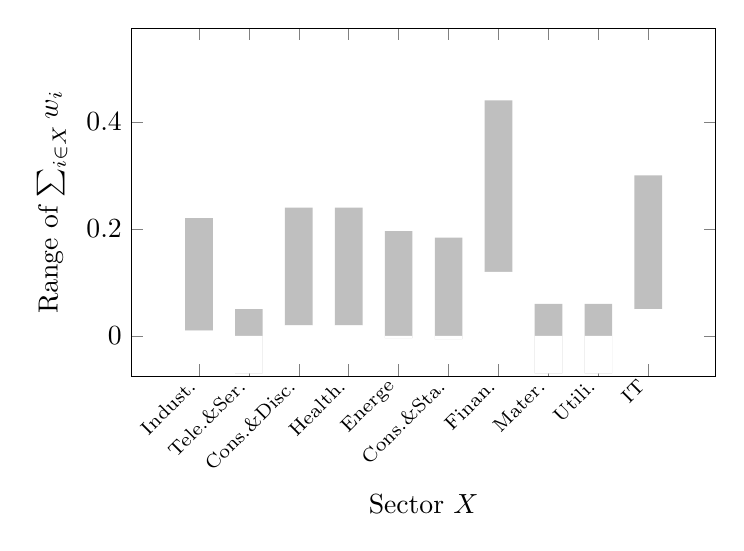
\begin{tikzpicture}
			\begin{axis}[
			width=9cm,
			height=6cm,
			ybar stacked,
			bar width=10pt,
			enlargelimits=0.15,
			legend style={at={(0.5,-1)},
				anchor=north,legend columns=-1},
			ylabel={Range of $\sum_{i \in X}w_i$},
			xlabel={Sector $X$},
			xlabel near ticks,
			ymin=0,
			ymax=0.5,
			symbolic x coords={Indust., Tele.\&Ser., Cons.\&Disc., Health., 
				Energe, Cons.\&Sta., Finan.,Mater.,Utili.,IT},
			xtick=data,
			x tick label style={rotate=45,anchor=east},
			xticklabel style = {font=\scriptsize}
			]
			
			\addplot+[ybar,color=black,draw=none,fill=white ] plot coordinates {(Indust., 0.01)
				(Tele.\&Ser., -0.07)
				(Cons.\&Disc., 0.02)
				(Health., 0.02)
				(Energe, -0.004)
				(Cons.\&Sta., -0.006)
				(Finan., 0.12)
				(Mater., -0.07)
				(Utili., -0.07)
				(IT, 0.05)
			};
			\addplot+[ybar,color=black, draw=none,fill=lightgray] plot coordinates { (Indust., 0.21)
				(Tele.\&Ser., 0.12)
				(Cons.\&Disc., 0.22)
				(Health., 0.22)
				(Energe, 0.2)
				(Cons.\&Sta., 0.19)
				(Finan., 0.32)
				(Mater., 0.13)
				(Utili., 0.13)
				(IT, 0.25)
			};
			
			\end{axis}
			\end{tikzpicture}
			\quad
			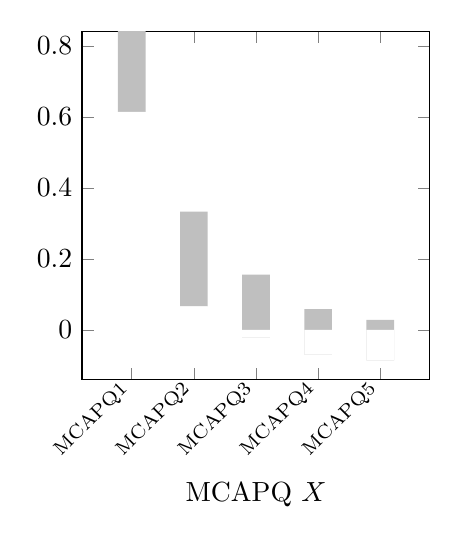
\begin{tikzpicture}
			\begin{axis}[
			width=6cm,
			height=6cm,
			ybar stacked,
			bar width=10pt,
			enlargelimits=0.2,
			legend style={at={(0.5,-1)},
				anchor=north,legend columns=-1},
			xlabel={MCAPQ $X$},
			xlabel near ticks,
			ymin=0,
			ymax=0.7,
			symbolic x coords={MCAPQ1, MCAPQ2, MCAPQ3, MCAPQ4, MCAPQ5},
			xtick=data,
			xticklabel style = {font=\scriptsize},
			x tick label style={rotate=45,anchor=east},
			]
			\addplot+[ybar,color=black,draw=none,fill=white ] plot coordinates {(MCAPQ1, 0.613783144)
				(MCAPQ2, 0.066327628)
				(MCAPQ3, -0.022)
				(MCAPQ4, -0.07)
				(MCAPQ5, -0.086)};
			\addplot+[ybar,color=black, draw=none,fill=lightgray] plot coordinates { (MCAPQ1, 0.81378314399999996)
				(MCAPQ2, 0.26632762799999998)
				(MCAPQ3, 0.17779934600000002)
				(MCAPQ4, 0.12814390000000001)
				(MCAPQ5, 0.113946004)	};
			\end{axis}
			\end{tikzpicture}
			\caption{The sum of the weights for each Sector and MCAPQ} \label{fig:sector:range}
		\end{center}
	\end{figure}
	Figure \ref{fig:sector:range} shows required sums of weights for sectors/MCAPQs to make constraints \eqref{eq:P:sector} and/or \eqref{eq:P:MCAPQ} with $w^{bench}$ for January 2007. Note that the required sums of weights are significantly varying for different sectors/MCAPQs. We calculate the required sum of weights for each of sectors/MCAPQs after selecting the leaving asset. If the any sum of weights is outside of the required range, we select the entering asset only among that sector/MCAPQ. Our computational experiments show that this selective choice of entering asset greatly increase the possibility of being feasible after the exchanging operation.
	
	
	
	
	
	
	%
	%
	%
	% infeasilbe cardinality sets occur in Constraints 7 and 8 indicating the limits of Sector Active Share and Market Cap Quintile (MCAPQ) Active Share.
	%
	%that when a QCQP problem is solved after fixing an asset with a cardinality set, a feasible solution can not be found in violation of some constraints. We have noticed that most infeasilbe cardinality sets occur in Constraints 7 and 8 indicating the limits of Sector Active Share and Market Cap Quintile (MCAPQ) Active Share.
	%	To see why, we took a look at data for the first date (date of January 3rd, 2007 ) of a given dataset. Figure 6 shows the sum of the weights for each sector and MCㅁAPQ to satisfy Constraints 6 and 7. Because $w_\text{bench} $ is different for each asset, the scope varies depending on what asset is included in the sector and the MCPQA. In other words, when the sum of each sector and MCAPQ is sensitive, it becomes a difficult constraint to satisfy. Therefore, if the constraints 6 and 7 are violated in the process of improving the cardinality set, adding deficient sector and mcapq assets is prevent infeasible. 
	%	
	%
	%
	%
	%
	%the local optimal solution may be improved depending on which asset is selected. Therefore, based on good initial cardinality set, it is necessary to perform a local search by changing the items of the asset, the weight of the asset, and the number of selected assets. However, if the initial cardinality set obtained from the GAN is not good in Step 1, changing the number of assets does not improve the result significantly. To determine the bad cardinality set, we check the quality of the solution when we solve the MIP with the initial cardinality set before updating the cardinality set. The following process is performed according to the result of 8 solutions. For 4 cardinality sets with bad results, it is required to find a new initial cardinality set ($\rightarrow$ Step1. Select Initial Cardinality Set). For 4 the other cardinality sets with good results, it adjusts the assets to improve results ($\rightarrow$ Step3. Update Algorithm). 
	%	
	%	%Update Algorithm
	%	
	%	\begin{figure}[h] 
	%		\begin{center}
	%			\includegraphics[width=0.65\textwidth]{step3}
	%			\caption{A Flowchart of Hybrid Approach} \label{fig:step3}
	%		\end{center}
	%	\end{figure}
	%	
	%	
	%	 Basically, update algorithm has 2 goals. 
	%	\begin{itemize}
	%		\item[(1)] One is that the update algorithm finds one or multiple assets whose objective value is lower when one or multiple assets is/are added or removed. 
	%		\item[(2)] The other is if the result of current cardinality set is infeasible, it also adjusts the cardinality set so that it becomes feasible.
	%	\end{itemize}
	%	To accomplish these two goals, the update aglrithm is supposed to adjust the cardinality set solving the problem and improving the solution until it is reachead to the end condition. First, the update algorithm finds out which asset gets better to lower the objective value when it gets out of the portfolio, and which asset should be added to improve the outcome. From the viewpoint of determining which asset is included in the portfolio, there is a great difficulty in deriving an objective value that can be obtained only when the weight of each asset is determined. We therefore take into account the maximum value that an asset has on the determination of the objective value. In the objective function, the risk is minimized while the return is maximized. Let $C$ is a set of assets whose asset $i$ is in cardinality set, and $K$ is a set of assets whose asset is not in cardinality set, that is candidate set for update algorithm. In order to find an good asset with higher return and lower risk, return and risk for the candidate asset $k \in K$ are calculated as follows:
	%	\begin{itemize}
	%		\item[\textbullet] Return = The maximum return that occurs as the asset $k$ comes in $\Rightarrow \alpha_k$
	%		\item[\textbullet] Risk = The maximum risk that occurs as the asset $k$ comes in $\Rightarrow \sum_{c \in C}\Omega_{ck} + \Omega_{kk}$
	%	\end{itemize}
	%	On the contrary, the asset $c$\textasciiacute$\,$ that increases the objective value because the risk is large and the return is small among the assets included in the current cardinality set is also determined by the following criteria : 
	%	\begin{itemize}
	%	\item[\textbullet] Return = The maximum return that decreases as the asset $c$\textasciiacute$\,$ leaves the cardinality set $\Rightarrow \alpha_{{c}'}$
	%	\item[\textbullet] Risk =  The maximum risk that decreases as the asset $c$\textasciiacute$\,$ leaves the cardinality set $\Rightarrow \sum_{c \in \{c | c \in C \, \text{and} \, c \neq \ {c}' \}}\Omega_{c {c}'} + \Omega_{{c}' {c}'}$
	%	\end{itemize}
	%	Therefore, in order to improve the objective function, the update algorithm minimizes the Risk $-$ Return for the new candidate asset $k$ and eliminates the asset $c$\textasciiacute$\,$ which have a bad effect on the existing cardinality set. Repeating this process can result in a local optimal solution as a result of obtaining a good cardinality set. However, infeasible cardinality sets can be obtained in many cases when considering the risk and return to obtain a good cardinality set. The cardinality set is infeasible, which means that when a QCQP problem is solved after fixing an asset with a cardinality set, a feasible solution can not be found in violation of some constraints. We have noticed that most infeasilbe cardinality sets occur in Constraints 7 and 8 indicating the limits of Sector Active Share and Market Cap Quintile (MCAPQ) Active Share.
	%	To see why, we took a look at data for the first date (date of January 3rd, 2007 ) of a given dataset. Figure 6 shows the sum of the weights for each sector and MCㅁAPQ to satisfy Constraints 6 and 7. Because $w_\text{bench} $ is different for each asset, the scope varies depending on what asset is included in the sector and the MCPQA. In other words, when the sum of each sector and MCAPQ is sensitive, it becomes a difficult constraint to satisfy. Therefore, if the constraints 6 and 7 are violated in the process of improving the cardinality set, adding deficient sector and mcapq assets is prevent infeasible. 
	%	
	\subsection{Detailed Description of Algorithm}
	%\subsection{GAN-MP Hybrid Approach} %이름 
	%We propose a new \textbf{GAN(Generative adversarial networks)-MP(Mathmatical Programming) Hybrid approach} that complements the disadvantages of formluation approach and neural network approach and enhances their advantages. Several limitations could be derived from the three approaches we present above. When solving the problem with the formulation appraoch, we could not find a reasonable solution because to consider about 500 assets per iteration the number of decision variables to decide and the number of constraints to be satisfied are too high . Especially, constraints (9) which select cardinalities considering the target range on number of stocks make the problem difficult. 
	%In the case of Neural Network Approach, there is a great advantage in that a solution that does not get significantly out from the whole constraints and that has a good objective value can be considered at the same time. However, it is difficult to find a soluton satisfying the feasibility for all the constraints and the fact that the training time takes too much time. The GAN-MP hybrid approach is a highly efficient approach that maximizes the advantages of GAN and formulation-based optimizations. This appraoch consists of three steps as shown in Figure 4. Step1 is the process of finding the cardinality set which is the combination of the selected assets. The cardinality set selected in Step1 solves the QCQP problem with the selected assets fixed and finds the local optimal solution in Step2. According to the result of Step2, the update algorithm finds cardinality set that can reduce the objective value and improves the solution.
	\begin{figure}[] 
		\begin{center}
			\includegraphics[width=0.45\textwidth]{flowchart}
			\caption{A Flowchart of Proposed Algorithm} \label{fig:flowchart}
		\end{center}
	\end{figure}
	Figure \ref{fig:flowchart} shows the flowchart of the proposed algorithm. The proposed algorithm greatly relies on the set of assets to invests that was generated by the GAN. Typically, the parameters of the GAN are initialized randomly. Because the training of NNs converges to local optima, different initialization values lead significantly distinct trained GANs. In other words, even though our GAN could take into account all constraints, the training of the GAN results in different local optima depending the starting conditions. To hedge this issue, we employed many independent GANs that were trained with different initial conditions (See Figure \ref{fig:parallelGAN}). For the parallel computing, we used Ipyparallel (\texttt{https://github.com/ipython/ipyparallel}) without any load balancing. 
	\begin{figure}[] 
		\begin{center}
			\includegraphics[width=0.6\textwidth]{step1}
			\caption{Parallel Training of Independent GANs} \label{fig:parallelGAN}
		\end{center}
	\end{figure}
	For example, on a 8-core machine we may spawn 8 independent GANs with distinct initialization parameters, which yields 8 considerably different sets of assets. Another aspect to consider regarding the training of GAN is which NN computation framework to use. We used PyTorch (\texttt{http://pytorch.org/}) for our experiments, and training time was less than 30 seconds using only 1 CPU core. We expect the training time can be reduced by using GPU or cloud computing service. 
	
	\begin{figure}[] 
		\begin{center}
			\includegraphics[width=0.65\textwidth]{step3}
			\caption{A Flowchart of Hybrid Approach} \label{fig:entire}
		\end{center}
	\end{figure}
	
	Figure \ref{fig:entire} illustrates the entire algorithm. When every process finishes Step 2, the obtained solutions are compared in the solution check stage. We pick top 50\% solutions in terms of the objective value and execute Step 3 on these solutions. For the remaining solutions, we discard them and initiate Step 1 from scratch with different initializers. The algorithm terminates when the given time limit (3 minutes) reaches. After finishing all procedures, the algorithm returns the best portfolio solution. 
	
	
	%	\underline{\textbf{(Step1) Select Initial Cardinality Set \& (Step2) Solve the QCQP }} :
	%	 When the number of assets to be considered is large, the problem becomes large as the number of constraints increases as well as decision variables. 
	%	 Thus, the process of step1 filters out good assets that are crucial for minimizing the objective value. At this time, the set of good assets must meet the following criteria.
	%	 \begin{itemize}
	%	 	\item[]\textbf{Criterion 1.} The combination of assets should be satisfy all constraints
	%	 	\item[]\textbf{Criterion 2.} The combination of assets is chosen to minimize the risk and maximize return.
	%	 \end{itemize}
	%	  In order to meet these criteria , the whole assets are required to be considered. We propose a formulation approach that finds the solution through Mixed Integer Programming (MIP) and a neural network-based GAN as a way to satisfy constraints and to take low values of objective value globally. Therefore, the experiments are carried out with two algorithms (MIP, GAN). For a given time, the MIP proceeds branch and bound(B\&B) and the GAN proceeds to train the generator consisting of NN (Step1). After the given time, the assets, $w_i> 0.001$ for all asset $i \in N$ ,were extracted in the best solution found in each algorithm. The portfolio optimization problem that determines the weight of each assets as the cardinality set is fixed (Step2) . Accordingly, constraints (9) does not to be considered anymore, and the set $N$ changes to $S$, which stands for set of selected assets for all of the constraints. Therefore, the number of constraints and decision varaibles are reduced. 
	% The following experiments were conducted to evaluate the performance of the algorithms.
	
	
	%
	%
	%	We present a model that can maximize the benefits of GAN in a given situation. The major advantage of the GAN is that it can extract solutions whenever noises are given to G by learning the weight and bias of the generator.
	%	The server that currently runs the code has eight cores, so we figure out the server can run up to 8 GANs simultaneously on 8 cores. Therefore, we use the parallel process to be 8 GANs training at the same time and then obtain 8 initial cardinality sets each as a result. The parallel process uses the Python Library of Ipython Parallel (https://ipyparallel.readthedocs.io), and Figure 6 shows the process of obtaining 8 sets of cardinality sets by running 8 GANs using Ipython Parallel.
	%
	%	\underline{\textbf{(Step3) Update Algorithm }} :  The assets to be included in the portfolio are selected by GAN, and the MIP is solved by Cplex for determining weights to each assets. 
	%	As a result of solving QCQP problems, the solutions are derived. At this time, the local optimal solution may be improved depending on which asset is selected. Therefore, based on good initial cardinality set, it is necessary to perform a local search by changing the items of the asset, the weight of the asset, and the number of selected assets. However, if the initial cardinality set obtained from the GAN is not good in Step 1, changing the number of assets does not improve the result significantly. To determine the bad cardinality set, we check the quality of the solution when we solve the MIP with the initial cardinality set before updating the cardinality set. The following process is performed according to the result of 8 solutions. For 4 cardinality sets with bad results, it is required to find a new initial cardinality set ($\rightarrow$ Step1. Select Initial Cardinality Set). For 4 the other cardinality sets with good results, it adjusts the assets to improve results ($\rightarrow$ Step3. Update Algorithm). 
	%	
	%	%Update Algorithm
	%	
	%	\begin{figure}[h] 
	%		\begin{center}
	%			\includegraphics[width=0.65\textwidth]{step3}
	%			\caption{A Flowchart of Hybrid Approach} \label{fig:step3}
	%		\end{center}
	%	\end{figure}
	%	
	%	
	%	 Basically, update algorithm has 2 goals. 
	%	\begin{itemize}
	%		\item[(1)] One is that the update algorithm finds one or multiple assets whose objective value is lower when one or multiple assets is/are added or removed. 
	%		\item[(2)] The other is if the result of current cardinality set is infeasible, it also adjusts the cardinality set so that it becomes feasible.
	%	\end{itemize}
	%	To accomplish these two goals, the update aglrithm is supposed to adjust the cardinality set solving the problem and improving the solution until it is reachead to the end condition. First, the update algorithm finds out which asset gets better to lower the objective value when it gets out of the portfolio, and which asset should be added to improve the outcome. From the viewpoint of determining which asset is included in the portfolio, there is a great difficulty in deriving an objective value that can be obtained only when the weight of each asset is determined. We therefore take into account the maximum value that an asset has on the determination of the objective value. In the objective function, the risk is minimized while the return is maximized. Let $C$ is a set of assets whose asset $i$ is in cardinality set, and $K$ is a set of assets whose asset is not in cardinality set, that is candidate set for update algorithm. In order to find an good asset with higher return and lower risk, return and risk for the candidate asset $k \in K$ are calculated as follows:
	%	\begin{itemize}
	%		\item[\textbullet] Return = The maximum return that occurs as the asset $k$ comes in $\Rightarrow \alpha_k$
	%		\item[\textbullet] Risk = The maximum risk that occurs as the asset $k$ comes in $\Rightarrow \sum_{c \in C}\Omega_{ck} + \Omega_{kk}$
	%	\end{itemize}
	%	On the contrary, the asset $c$\textasciiacute$\,$ that increases the objective value because the risk is large and the return is small among the assets included in the current cardinality set is also determined by the following criteria : 
	%	\begin{itemize}
	%	\item[\textbullet] Return = The maximum return that decreases as the asset $c$\textasciiacute$\,$ leaves the cardinality set $\Rightarrow \alpha_{{c}'}$
	%	\item[\textbullet] Risk =  The maximum risk that decreases as the asset $c$\textasciiacute$\,$ leaves the cardinality set $\Rightarrow \sum_{c \in \{c | c \in C \, \text{and} \, c \neq \ {c}' \}}\Omega_{c {c}'} + \Omega_{{c}' {c}'}$
	%	\end{itemize}
	%	Therefore, in order to improve the objective function, the update algorithm minimizes the Risk $-$ Return for the new candidate asset $k$ and eliminates the asset $c$\textasciiacute$\,$ which have a bad effect on the existing cardinality set. Repeating this process can result in a local optimal solution as a result of obtaining a good cardinality set. However, infeasible cardinality sets can be obtained in many cases when considering the risk and return to obtain a good cardinality set. The cardinality set is infeasible, which means that when a QCQP problem is solved after fixing an asset with a cardinality set, a feasible solution can not be found in violation of some constraints. We have noticed that most infeasilbe cardinality sets occur in Constraints 7 and 8 indicating the limits of Sector Active Share and Market Cap Quintile (MCAPQ) Active Share.
	%	To see why, we took a look at data for the first date (date of January 3rd, 2007 ) of a given dataset. Figure 6 shows the sum of the weights for each sector and MCㅁAPQ to satisfy Constraints 6 and 7. Because $w_\text{bench} $ is different for each asset, the scope varies depending on what asset is included in the sector and the MCPQA. In other words, when the sum of each sector and MCAPQ is sensitive, it becomes a difficult constraint to satisfy. Therefore, if the constraints 6 and 7 are violated in the process of improving the cardinality set, adding deficient sector and mcapq assets is prevent infeasible. 
	
	
	
	\section*{Analytics Solution and Results}
	\setcounter{subsection}{0}
	
	\subsection{Experiments for Each Step}
	
	The proposed algorithm has a sequential process and roles assigned to each step are as follows:
	\begin{itemize}
		\item Step 1: Populating good initial sets of assets (GAN).
		\item Step 2: Obtaining feasible solutions under the given set of assets (Bisectional search algorithm).
		\item Step 3: Improving feasible solutions obtained at the previous step (Local search algorithm).
	\end{itemize}
	
	In this section, we report computational results that confirm validity of each step. 
	
	
	%	to derive the (near) optimal solution.  Note that we present steps to solve the portfolio optimization, and each steps can be specified as follows:
	%First, we show how to set the parameter $\lambda$ to be considered in the problem in order to obtain the optimal solution before proceeding with the experiment. Also, we present how rebalancing reflects in our proposed model. Finally, the results of the computational experiments with the determined parameters are present.
	
	
	\subsubsection{Step 1 : Select Initial Set of Assets }
	
	We conducted the following experiments to show the performance of our GAN-based initial set selection process. We compared the GAN-based approach to a simple random set selection method. The experiment settings are as follows:
	\begin{itemize}
		\item Number of experiments : 50 times
		\item Training time for GAN : 20 seconds
		\item Neural network library : PyTorch (\texttt{http://pytorch.org/})
		\item Data of the first period (January 2007)
		\item Baseline method: randomly selecting 60 assets for each initial set
	\end{itemize}
	
	\begin{figure}[]
		\begin{center}
			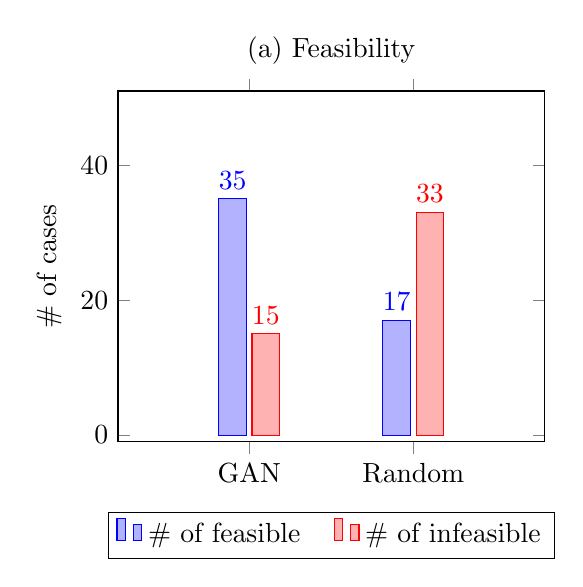
\begin{tikzpicture}[scale=1]
			\begin{axis}[
			ybar,
			enlargelimits=0.8,
			legend style={at={(0.5,-0.20)},
				anchor=north,legend columns=-1},
			ylabel={\# of cases},
			symbolic x coords={GAN, Random},
			xtick=data,
			nodes near coords,
			nodes near coords align={vertical},
			title={(a) Feasibility}
			]
			\addplot coordinates { (GAN,35) (Random,17)};
			\addplot coordinates { (GAN,15) (Random,33)};
			\legend{\# of feasible$\quad$, \# of infeasible}
			
			\end{axis}
			\end{tikzpicture} 
			\quad
			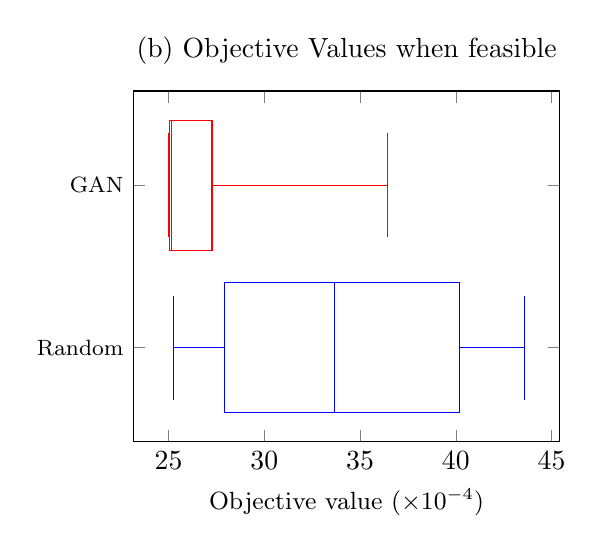
\begin{tikzpicture}[scale=1.]
			\begin{axis}
			[
			ytick={1,2},
			yticklabels={\footnotesize Random, \footnotesize GAN},
			xlabel={\small Objective value ($\times 10^{-4}$)},
			title={(b) Objective Values when feasible}
			]
			
			\addplot+[
			boxplot prepared={
				median=33.66,
				upper quartile=40.18,
				lower quartile=27.90,
				upper whisker=43.58,
				lower whisker=25.26
			},
			] coordinates {};
			\addplot+[
			boxplot prepared={
				median=25.14,
				upper quartile= 27.27,
				lower quartile=25.056,
				upper whisker=36.43,
				lower whisker=25.013
			},
			] coordinates {};
			
			\end{axis}
			\end{tikzpicture}
			\caption{Experiments Results for Step 1} \label{fig:step1}
		\end{center}
	\end{figure}
	
	We injected the populated sets from two methods into Step 2 (Bisectional search algorithm), and evaluated the feasibility and objective values if feasible. Figure \ref{fig:step1} compares the results of two methods. The numbers of feasible cases vs. infeasible cases out of 50 trials are shown in Figure \ref{fig:step1}(a). It is clearly shown that the GAN-based approach outperforms the random selector. When a feasible set is found, the expected objective value is much better for the GAN-based approach as shown in Figure \ref{fig:step1}(b).
	
	\underline{Insights and Suggestion:} the GAN is composed of NNs, and the quality of results, especially training time, heavily depend on computing environment. Therefore, we recommend that Principal could improve the training speed and quality by using GPU-accelerated computing or through some advanced technologies such as Amazon Cloud services. Moreover, the structure of generator \textbf{G} is worth of further investigating because the numbers of hidden layers and units are of crucial importance in training of GAN. We also found that the fully-trained GANs often produce considerably different initial sets because of different initial conditions. We would recommend employing parallel training of multiple GANs with distinct initial parameters, which results in much divergent initial sets. 
	
	
	% By improving the environment, more accurate and better solutions are derived by adjusting the hidden layer addition and the learning rate that we could not reflect now because of computing power. 
	
	%	The process of step1 filters out good assets that are crucial for minimizing the objective value. In section 2, we propose an GAN based algorithm for selecting initial set of assets to invest. The following experiment was conducted to confirm that the GAN works well.
	%	
	%	\begin{itemize}
	%		\item Experiment Results :
	%
	%		\item[]  As a result of the experiment, the initial sets of assets generated by using GAN not only finds feasible solution well but the objective value which solved with the feasible solution is much lower. Therefore ,we derive better solutions by obtaining initial set of assets using GAN.
	%		
	%		\item Threshold and Suggestion :
	%		GAN is composed of NNs, and the result quality and training time vary depending on computing environment of NN. Therefore, we recommend that Principal could improve the training speed and quality by using GPU-accelerated computing or through some advanced technologies such as Amazon Cloud services. By improving the environment, more accurate and better solutions are derived by adjusting the hidden layer addition and the learning rate that we could not reflect now because of computing power. 
	%		
	%	\end{itemize}
	
	
	\subsubsection{Step2 : Solving (P2) \& Bisectional Search }
	
	In Step 2, we solve the convex QCQP problem (P2) with a given set of assets $\hat{N}$. Because the problem (P2) relaxes two non-convex constraints, we need to warrant the feasibility of the solution obtained. As we stated before, we do a bisectional search to find a feasible solution by increasing the sum of weights of a subset assets. Figure \ref{fig:bisectional search} shows the changes of the TE and AS values during the search algorithm. We found that the AS values are rarely violating the constraint (red line in the figure), while the TE values are typically well below from the required lower bound. In Figure \ref{fig:bisectional search}, is is shown that the TE values are fluctuating significantly because of the added constraint \eqref{eq:P2:bs}. The black squares represent finding of feasible solutions. It is evident that during the bisectional search, many feasible solutions can be found. We return the feasible solution with the best objective value.
	
	%	the results which finds the feasible solution through bisectional search. As the bisectional search is repeated, it is confirmed that the tracking error converges to the lower bound(0.25). Accordingly, the feasible solution is derived.
	
	\begin{figure}[h]
		\begin{center}
			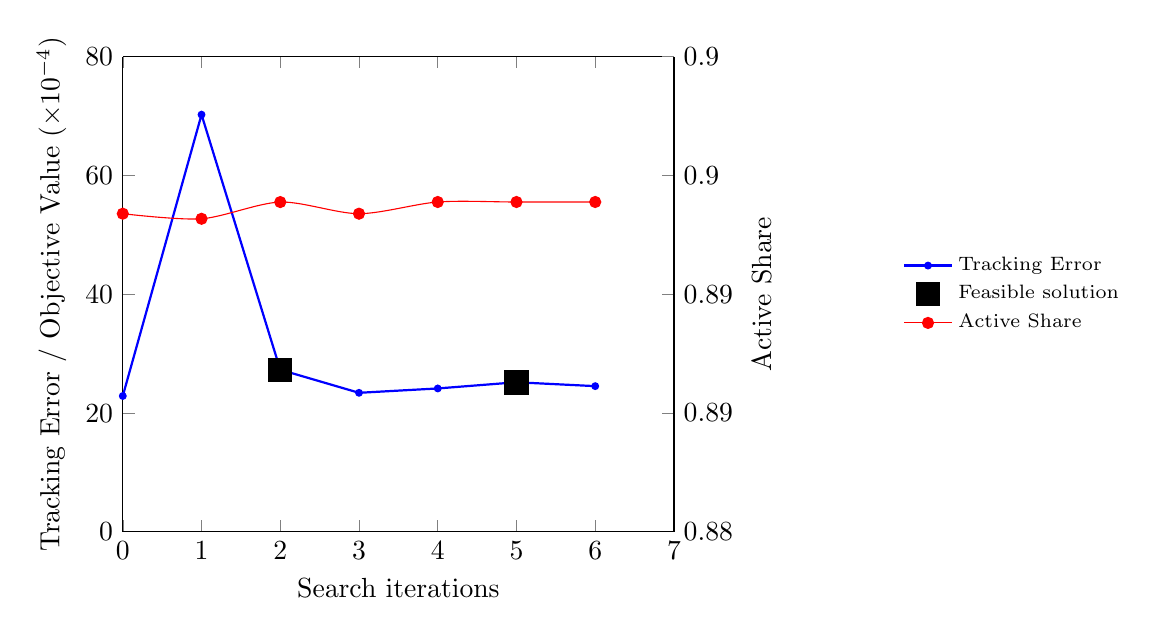
\begin{tikzpicture}[scale=1]
			\begin{axis}[
			scale only axis,
			axis y line*=left,
			xmin=0, xmax=7,
			ymin=0, ymax=80,
			xlabel=Search iterations,
			ylabel={Tracking Error / Objective Value ($\times 10^{-4}$)},
			legend style={draw=none, font=\scriptsize},
			legend cell align=left,
			legend style={at={(1.4,0.5)}, anchor=west},
			%label style={font=\scriptsize},
			legend entries={{Tracking Error}, {Feasible solution},{Active Share}}]
			\addplot[color=blue, thick, mark=*,mark options={scale=0.5}] coordinates {
				(0, 22.87835501)
				(1, 70.22758985)
				(2, 27.29357997)
				(3, 23.41346661)
				(4, 24.14684022)
				(5, 25.18932616)
				(6, 24.53572075) };
			%\addlegendentry{TE}
			\addplot[black,scatter,only marks,  scatter/classes={a={mark=square*,black}},mark=square*, thick,mark options={scale=2}] coordinates {
				%	(0, 22.82923962950044)
				(2, 27.246690713625878)
				%	(3, 23.363384835018515)
				%	(4, 24.096623164811717)
				(5, 25.14073766356739)
				%	(6, 24.486286272271638)
			};
			%scatter src=explicit symbolic]
			\addplot[smooth,mark=*,red] 
			coordinates{(10,1)
			};
			%\legend{$\eta$}
			\end{axis}
			
			\begin{axis}[
			scale only axis,
			/pgf/number format/sci subscript,
			axis y line*=right,
			axis x line=none,
			xmin=0, xmax=7.,
			ymin=0.88, ymax=0.9,
			ylabel=Active Share]
			\addplot[smooth,mark=*,red] 
			coordinates{
				(0, 0.893388450961)
				(1, 0.893174573)
				(2, 0.893877522666)
				(3, 0.893388448546)
				(4, 0.893880492111)
				(5, 0.893879951624)
				(6, 0.893880528913)
			};
			%\addlegendentry{$\eta$}
			%\legend{$\eta$}
			\end{axis}
			
			\end{tikzpicture}
			\caption{The Results of Bisectional Search} \label{fig:bisectional search}
		\end{center}
	\end{figure}
	
	\underline{Insights and Suggestion:} Even the bisectional search is able to find good feasible solutions quickly, the added constraint \eqref{eq:P2:bs} can make the feasible solutions somewhat restrictive because the set of assets to increase $N^+$ is fixed. One can try different choice for $N^+$, or update the set $N^+$ on the fly during search. 
	
	
	\subsubsection{Step 3: Local Search for Improving Solutions}
	
	The feasible solution obtained from Step 2 is improved in this step. A good asset that might reduce the objective value is identified by \eqref{eq:entering}, and added to the current set of assets to invest. Conversely, the asset that might make the objective value higher is removed by using \eqref{eq:leaving}. Figure \ref{fig:local search} shows the changes of objective values of the solutions with repeating the exchanging operations for 60 seconds. It is clear that the objective values are kind of ``saturated'' around 0.0025. This behavior is because the term $d^T \Omega d$ approaches to 0.0025 due to the TE constraint \eqref{eq:P:TE}. We found that compared to $d^T \Omega d$, another term in the objective function $d^T \alpha$ contribute very little, which results in the objective values of many good solutions being around 0.0025. 
	
	\begin{figure}[h]
		\begin{center}
			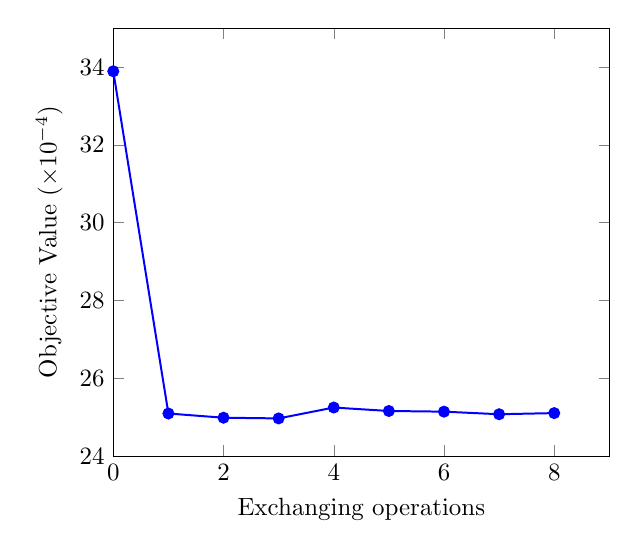
\begin{tikzpicture}[scale=0.9]
			\begin{axis}[
			scale only axis,
			xmin=0, xmax=9,
			ymin=24, ymax=35,
			xlabel=Exchanging operations,
			ylabel={Objective Value ($\times 10^{-4}$)}]
			%legend style={draw=none, font=\scriptsize},
			%legend cell align=left,
			%legend style={at={(0.5,-0.25)}, anchor=north},
			%label style={font=\scriptsize},
			%legend entries={{Tracking Error}, {Objective Value},{Active Share}}]
			\addplot[color=blue, thick, mark=*, mark options={scale=1}] coordinates {
				(0, 33.891587285731134)
				(1, 25.09299329561036)
				(2, 24.984764546200704)
				(3, 24.966975825718855)
				(4, 25.24671235679147)
				(5, 25.158038999590666)
				(6, 25.14073766356739)
				(7, 25.0744257270579)
				(8, 25.103619932228014)};
			%\addlegendentry{TE}
			
			%scatter src=explicit symbolic]
			
			%\legend{$\eta$}
			\end{axis}
			\end{tikzpicture}
			\caption{The Results of Local Search} \label{fig:local search}
		\end{center}
	\end{figure}
	
	
	\underline{Insights and Suggestion:} The given scaling choice of $\Omega$ and $\alpha$ implies that the ``true'' optimal portfolio should be those with minimum risk. That is, even the objective function has two terms for the risk and return, the risk should be considered more seriously than the return. This observation motivates a goal programming based approach. For example, we may add constraint $d^T \Omega d \le 0.0025 + \epsilon$, and maximize only the return $d^T \alpha$, where $\epsilon$ is a very small value.
	
	
	
	
	
	
	
	\subsection{Computational Experiments}
	In this section, we report results of computational experiments for solving portfolio optimization with the methodology we present. 
	%Experimental data is used and future data were not used based on the time of experiment. 
	The experiment was conducted with the provided data, and no future data was used at the point time concerned. For every rebalance to rebalance, maximum of 3 minutes of computational time was used for the whole computation. 
	
	\underline{\textbf{Experiment environment}} : The experiments were performed on an Intel Xeon 3.5 GHz MacPro machine with 32GB memory and ILOG CPLEX 12.6 were used as an MIP solver, and PyTorch for Python 3.6 was used as a deep learning framework. 
	
	\underline{\textbf{Computational Results}} : The experiment was performed for all given periods, and Table \ref{computational} shows the results of experiment for the year of 2007. In most cases, the objective value is close to the lower bound of the tracking error, which is restricted by constraint \eqref{eq:P:TE}. Therefore, we might say our solution is near optimal. On the other hand, the value of $ r_{opt}$, calculated by the product of the actual return $r$, and the portfolio weight $w$ is relatively irregularly formed. The execution time for the proposed algorithm is also shown in the table. The execution time of Step 1, which is the process of selecting the initial set of assets using the GAN, includes the time for forming the network and the training time. Step 2 includes the setup and formulating time to solve (P2) and the time for the branch and bound by CPLEX, and the execution time of Step 3 contains all the time that occurs in the process of improving the solution by doing a local search. Therefore, we ensure that the proposed algorithm produces relatively good solutions in a rather short execution time (< 3 minutes). We note that the MacPro machine used for the experiments only has 6 CPU cores, which may deteriorate the computational times because we spawned total 8 processes. A more powerful machine would allow us to spend more time in each step, which would improve the quality of solutions.
	
	\begin{table}[]
		\centering
		\caption{The Computational Results of the Algorithm Proposed (year of 2007)}
		\label{computational}
		\resizebox{\textwidth}{!}{%
			\begin{tabular}{cccccccccccccc}
				\multicolumn{1}{l}{} & \multicolumn{1}{l}{} & \multicolumn{1}{l}{} & \multicolumn{1}{l}{} & \multicolumn{1}{l}{} & \multicolumn{1}{l}{} & \multicolumn{1}{l}{} & \multicolumn{1}{l}{} & \multicolumn{1}{l}{} & \multicolumn{1}{l}{} & \multicolumn{1}{l}{} & \multicolumn{1}{l}{} & \multicolumn{1}{l}{} & \multicolumn{1}{l}{} \\ \toprule
				\multicolumn{2}{c}{\textbf{Instance}} &  & \multicolumn{5}{c}{\textbf{Output}} &  & \multicolumn{5}{c}{\textbf{Execution Time (sec)}} \\[1mm]  \cline{1-2} \cline{4-8} \cline{10-14} 
				Date & \# of asset & \textbf{} & \begin{tabular}[c]{@{}c@{}}\# of assets \\ to invest\end{tabular} & \begin{tabular}[c]{@{}c@{}}Objective \\ Value\end{tabular} & $r_{Txadj t}$ & $r_{opt t}$ & turnover & \textbf{} & \begin{tabular}[c]{@{}c@{}}Pre\\ -processing\end{tabular} & Step1 & Step2 & Step3 & Total \\
				\midrule
				01/31/2007 & 493 &  & 70 & 30.81 & 0.005 & 0.011 & 1.116 &  & 0.269 & 53.09 & 71.12 & 44.37 & 168.86 \\
				02/28/2007 & 494 &  & 70 & 30.80 & -0.016 & -0.011 & 1.107 &  & 0.274 & 53.35 & 70.18 & 42.78 & 166.59 \\
				03/28/2007 & 494 &  & 70 & 31.02 & -0.005 & 0.0005 & 1.193 &  & 0.275 & 53.17 & 70.56 & 43.39 & 167.41 \\
				04/25/2007 & 494 &  & 70 & 30.75 & 0.047 & 0.052 & 1.034 &  & 0.276 & 53.29 & 70.6 & 43.84 & 168.02 \\
				05/23/2007 & 494 &  & 64 & 29.56 & 0.019 & 0.023 & 0.776 &  & 0.272 & 53.18 & 71.79 & 44.61 & 169.87 \\
				06/20/2007 & 494 &  & 60 & 31.82 & -0.009 & -0.003 & 1.322 &  & 0.277 & 53.13 & 70.35 & 42.13 & 165.90 \\
				07/18/2007 & 493 &  & 70 & 31.88 & -0.001 & 0.006 & 1.351 &  & 0.284 & 53.35 & 70.19 & 43.97 & 167.81 \\
				08/15/2007 & 493 &  & 70 & 30.47 & -0.071 & -0.066 & 1.030 &  & 0.271 & 57.14 & 72.15 & 44.46 & 174.04 \\
				09/12/2007 & 493 &  & 70 & 29.93 & 0.019 & 0.024 & 0.932 &  & 0.277 & 53.19 & 70.39 & 44.04 & 167.90 \\
				10/10/2007 & 495 & \multicolumn{1}{l}{} & 70 & 30.52 & 0.084 & 0.089 & 1.063 & \multicolumn{1}{l}{} & 0.274 & 53.20 & 70.09 & 42.57 & 166.15 \\
				11/07/2007 & 495 & \multicolumn{1}{l}{} & 70 & 30.32 & -0.064 & -0.059 & 1.062 & \multicolumn{1}{l}{} & 0.277 & 53.26 & 71.08 & 44.19 & 168.81 \\
				12/05/2007 & 495 & \multicolumn{1}{l}{} & 70 & 30.15 & -0.009 & -0.005 & 0.91 & \multicolumn{1}{l}{} & 0.276 & 53.15 & 70.98 & 42.68 & 167.10 \\
				\cline{1-2} \cline{4-8} \cline{10-14} 
				\multicolumn{2}{c}{\textbf{Mean}} & \multicolumn{1}{l}{} & \textbf{68.66} & \textbf{30.67} & \textbf{-0.0003} & \textbf{0.005} & \textbf{1.075} & \multicolumn{1}{l}{} & \textbf{0.275} & \textbf{53.54} & \textbf{70.79} & \textbf{43.59} & \textbf{168.20} \\
				\bottomrule
			\end{tabular}%
		}
	\end{table}
	
	\underline{\textbf{The Portfolio Performance Statistics}} :  The portfolio performance statitstics below is averaged over 10 years of data.
	\begin{center}
		\textbf{Portfolio Performance Statistics}\vspace*{-14pt}
	\end{center}
	
	\begin{table}[htbp]
		\def\arraystretch{1.4}
		\begin{center}
			\begin{tabular}{|l|c|c|}
				\hline
				\textbf{2007-01-01 to 2016-12-31}& 
				\textbf{Portfolio}& 
				\textbf{Benchmark} \\
				\hline
				Cumulative Return& 
				{13.1\%}& 
				{20.3\%} \\
				\hline
				Annualized Return& 
				{13.1\%}& 
				{20.3\%} \\
				\hline
				Annualized Excess Return& 
				{-7.3\%}& 
				-- \\
				\hline
				Annualized Tracking Error& 
				{3.7\%}& 
				-- \\
				\hline
				Sharpe Ratio& 
				3.8& 
				\\
				\hline
				Information Ratio& 
				-7.8& 
				-- \\
				\hline
			\end{tabular}
			\label{tab1}
		\end{center}
	\end{table}
	
	
	
	
	\subsection{Parameter Setting}
	Out approach provides many algorithmic parameters. Ideally, to optimally tune parameters, various experimental analyzes are required with real data. However, given limited information on construction methods of the data such as $\alpha, \Omega, \beta$, and bench weights. We assume that the year of 2007 is a parameter adjustment period, and adjusted our parameters based on the results of 2007. Note that for the year of 2007, we simply used default values (e.g., 1) for all parameters, because we are now allowed to use the future outcomes to tune the past portfolios. 
	
	\underline{\textbf{The Parameter $\lambda$}}: Parameter $ \lambda $ reflects how much return will be considered relative to risk in the objective function. When the value of $ \lambda $ is large, the return is supposed to be considered more, and when the $\lambda$ value is small, the risk is considered more. We used results of the year of 2007 to analyze whether the $d^{T} \alpha$, which represents the return, has an influence on the overall return index ($r_{opt}$) as we adjusted the $\lambda$. In other words, as the $\lambda$ value increases, more revenue will be taken into account, so that it can be inferred that the $r_{opt}$  is more affected by return or risk. Therefore, we conduct the simulation by changing $ \lambda $ with the first year of data. Then, we compare the experimental result with the actual return value to see how much the parameter $ \lambda $ affects the overall return. Experimental results show that the distribution of $r_{opt}$  is not affected by $\lambda$ values. We believe the causes of the experimental results as follows: First, the scale of $\alpha$ which is an index of return, and the scale of $\Omega$ which is an index of risk, are very different in the objective function. In other words, the $\alpha$ is too small, so even if the parameter $\lambda$ is 10, return is still considered small. The second reason is that there is a very low correlation between $\alpha$ and $r$, further consideration of $\alpha$ does not improve actual returns. 
	\begin{figure}[h] 
		\begin{center}
			\includegraphics[width=0.55\textwidth]{lambda}
			\caption{ Kernel Density Estimation according to $\lambda$ } \label{fig:lambda}
		\end{center}
	\end{figure}
	
	\subsection{Rabalancing}
	
	Portfolio turnover depends on how many assets in the portfolio change from rebalance to rebalance, and the value of turnover has effects on Information Ratio (IR). Therefore, it is required to consider turnover in the portfolio optimization. We apply additional consideration for the turnover to the both GAN for finding initial  set of assets and the QCQP problem for determining the weight of the selected assets. For applying it to GAN, the calculated $\text{turnover}_{t} (\sum_{i \in N}|w_{i,t}-w_{i,t-1}^{pre}|)$ was added to the loss function of the discriminator \textbf{D}. On the other hand, for applying it to (P2), it should be linearized, which results in the following formulation:
	\begin{align*}
	\text{(P2-TO)} \quad \min~ & d^T\Omega d  -  \lambda d^{T}\alpha + \omega \sum_{i \in N}o_i \\
	\text{s.t. } 
	& \eqref{eq:P:activeweight}, \eqref{eq:P:nonn} - \eqref{eq:P:beta}, \notag\\
	& w_i \le 0, & \forall i \in N \backslash \hat{N}, \\
	& w_i \geq 0.001, & \forall i \in \hat{N}, \\
	& d^T \Omega d \leq 0.01. \\
	& o_i \geq w_{i,t}-w_{i,t-1}^{pre}, & \forall{i \in N} \\
	& o_i \geq -w_{i,t}+w_{i,t-1}^{pre}, & \forall{i \in N} 
	\end{align*} 
	The decision variables $o_i$ is the difference between $w_i$ of previous period $(t-1)$ and $w_i$ of current($t$) period for all asset $i \in N$. Because of constraints added, $ w_{i,t}-w_{i,t-1}^{pre}$ is positive for all asset $i \in N$. The parameter $\omega$ represents the weight of turnover for objective value considering risk and return. 
	
	\underline{\textbf{The Parameter $ \omega$}}: Experiment with a large value of $ \omega $ considers turnover a lot when compared to risk-return. In the opposite side, the turnover cost is significant. Since our computational experimence with the year of 2007 showed that $\omega=5$ would yield decent results, we set $\omega=5$ in the following years.
	
	
	%실험내용
	%실험결과 및 결론
	
	
	\subsection{Dealing Uncertainty of $\alpha$} 
	
	The results obtained earlier are derived by deterministic values which are $\alpha$ and $\Omega$. However, this is a parameter value with uncertainty, so we figure out the change of $\alpha$ and $\Omega$ in the historical data.  We first tried to secure the value of risk and alpha score for 2007 by analyzing the historical data. The analyzed data is obtained from Yahoo Finance and is historical data from 1970 to 2017. For the first time, we are looking at the risk of an asset in 2006 with extensive historical data. We obtained data on close stock prices for approximately 400 assets from historical data among 492 assets included in January 3, 2007 in S \& P 500 and derived a cross covariance matrix. And then, the correlation between the covariance matrix and the full matrix of $\Omega$ was derived. We expected a large correlation between the two matrices, but the result was not. It is judged that it is difficult to deduce $\Omega$ value from the covariance matrix derived from historical data. Therefore, we obtain the range of parameter change for each asset with the first year data received from the Principal and reflect it in the following robust optimization. %왜 \alpha만 고려하는가? 쉽게 고려할 수 있는 부분?
	
	Let set $U := \{ \tilde \alpha \in \mathbb{R}^{|N|}  \mid \tilde \alpha_i = \alpha_i + \bar{\alpha}_i \gamma_i , \quad -1 \leq \gamma_i\leq 1 , \quad \sum_{i} |\gamma_i| = \Gamma \}$, which contains all possible realizations of $\alpha$. Our goal is to consider the worst-case realization of $U$, which means that the expected return of the active weight ($d^T \tilde{\alpha}$) is guaranteed above the worst-case value. The mathematical formulation addressing the uncertainty of $\alpha$ is stated as follows:
	\begin{align}
	\text{(RP)} \quad \min~ & d^T \Omega d - \lambda \min_{\tilde{\alpha} \in U} \{d^T \tilde{\alpha} \} \label{eq:RP:obj}\\
	\text{s.t. } 
	& \eqref{eq:P:activeweight}, \eqref{eq:P:nonn} - \eqref{eq:P:TE}. \notag
	\end{align}
	For a given $d$, the inner minimization problem is stated as
	\begin{align}
	\min_{\tilde{\alpha} \in U} \{ d^T \tilde{\alpha} \} &= \min \left\{ \sum_{i \in N} d_i (\alpha_i + \bar{\alpha}_i \gamma_i ) : -1 \le \gamma_i \le 1, \forall i \in N, \sum_{i \in N} |\gamma_i| = \Gamma  \right\}\\
	&= d^T \alpha - \max \left\{ \sum_{i \in N} |d_i| \bar{\alpha}_i \gamma_i : 0 \le \gamma_i \le 1, \forall i \in N, \sum_{i \in N} \gamma_i = \Gamma  \right\}.
	\end{align}
	As shown by \cite{bertsimas2004price}, the latter maximization problem has an integral polyhedron. Using the linear programming duality theory, it is easily shown that the following holds:
	\begin{align}
	&\max \left\{ \sum_{i \in N} |d_i| \bar{\alpha}_i \gamma_i : 0 \le \gamma_i \le 1, \forall i \in N, \sum_{i \in N} \gamma_i = \Gamma  \right\} =\\
	&\min \left\{ \Gamma \pi + \sum_{i \in N} \theta_i : \pi + \theta_i \ge \bar{a}_i p_i,~ -p_i \le d_i \le p_i,~ \theta_i \ge 0, ~\forall i \in N   \right\}
	\end{align}
	Then, the problem (RP) can be reformulated as
	\begin{align}
	\text{(RP1)} \quad \min~ & d^T \Omega d - \lambda \left[ d^T \alpha - \left(\Gamma \pi + \sum_{i \in N} \theta_i \right) \right] \label{eq:RP1:obj}\\
	\text{s.t. } 
	& \eqref{eq:P:activeweight}, \eqref{eq:P:nonn} - \eqref{eq:P:TE}, \notag\\
	& \pi + \theta_i \ge \bar{\alpha}_i p_i, & \forall i \in N, \\
	& -p_i \le d_i \le p_i, & \forall i \in N,\\
	& \theta_i \ge 0, & \forall i \in N.
	\end{align}
	Note that (RP1) reduces to the problem (P) when $\Gamma=0$. Because reformulation of (RP1) involves only linear constraints and continuous decision variables, the proposed algorithm for (P) can be used for solving (RP1) without further modifications except the mathematical formulation. 
	\begin{table}[]
		\centering
		\caption{The Comparision of Performance about $\Gamma$  }
		\label{gamma}
		\begin{tabular}{cccccccccc}
			&  &  &  &  &  &  &  &  &  \\ \hline
			&  & \multicolumn{2}{c}{Output} &  & \multicolumn{5}{c}{Execution Time (sec)} \\[1mm] \cline{3-4} \cline{6-10} 
			&  & IR & rTxadjt &  & Pre-processing & Step1 & Step2 & Step3 & Total \\ \cline{1-1} \cline{3-10} 
			$\gamma$ = 0 &  & -3.47 & 0.005 &  & 0.28 & 35.53 & 84.49 & 44.27 & 164.59 \\
			$\gamma$ = 5 &  & -1.32 & 0.007 &  & 0.26 & 32.61 & 141.34 & 29.04 & 203.27\\ \hline
		\end{tabular}
	\end{table}
	
	
	
	\bibliographystyle{chicago}
	\bibliography{informs}
	
	
\end{document}
